\section{Attack}\label{sec:attack}

\begin{figure*}
    \centering
    \begin{subfigure}{.18\textwidth}
        \centering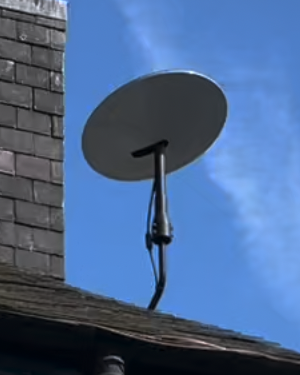
\includegraphics[width=\textwidth]{img/unstowed.png}\\\vspace{.35em}
        \centering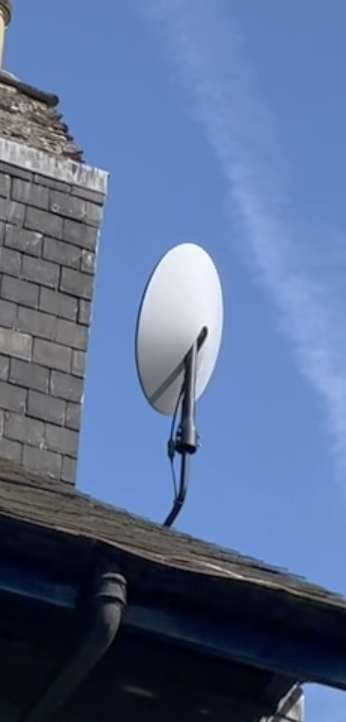
\includegraphics[width=\textwidth]{img/stowed.png}
        \caption{The dish in ``active'' and ``stowed'' modes.}
    \end{subfigure}
    \begin{subfigure}{.52011\textwidth}
        \centering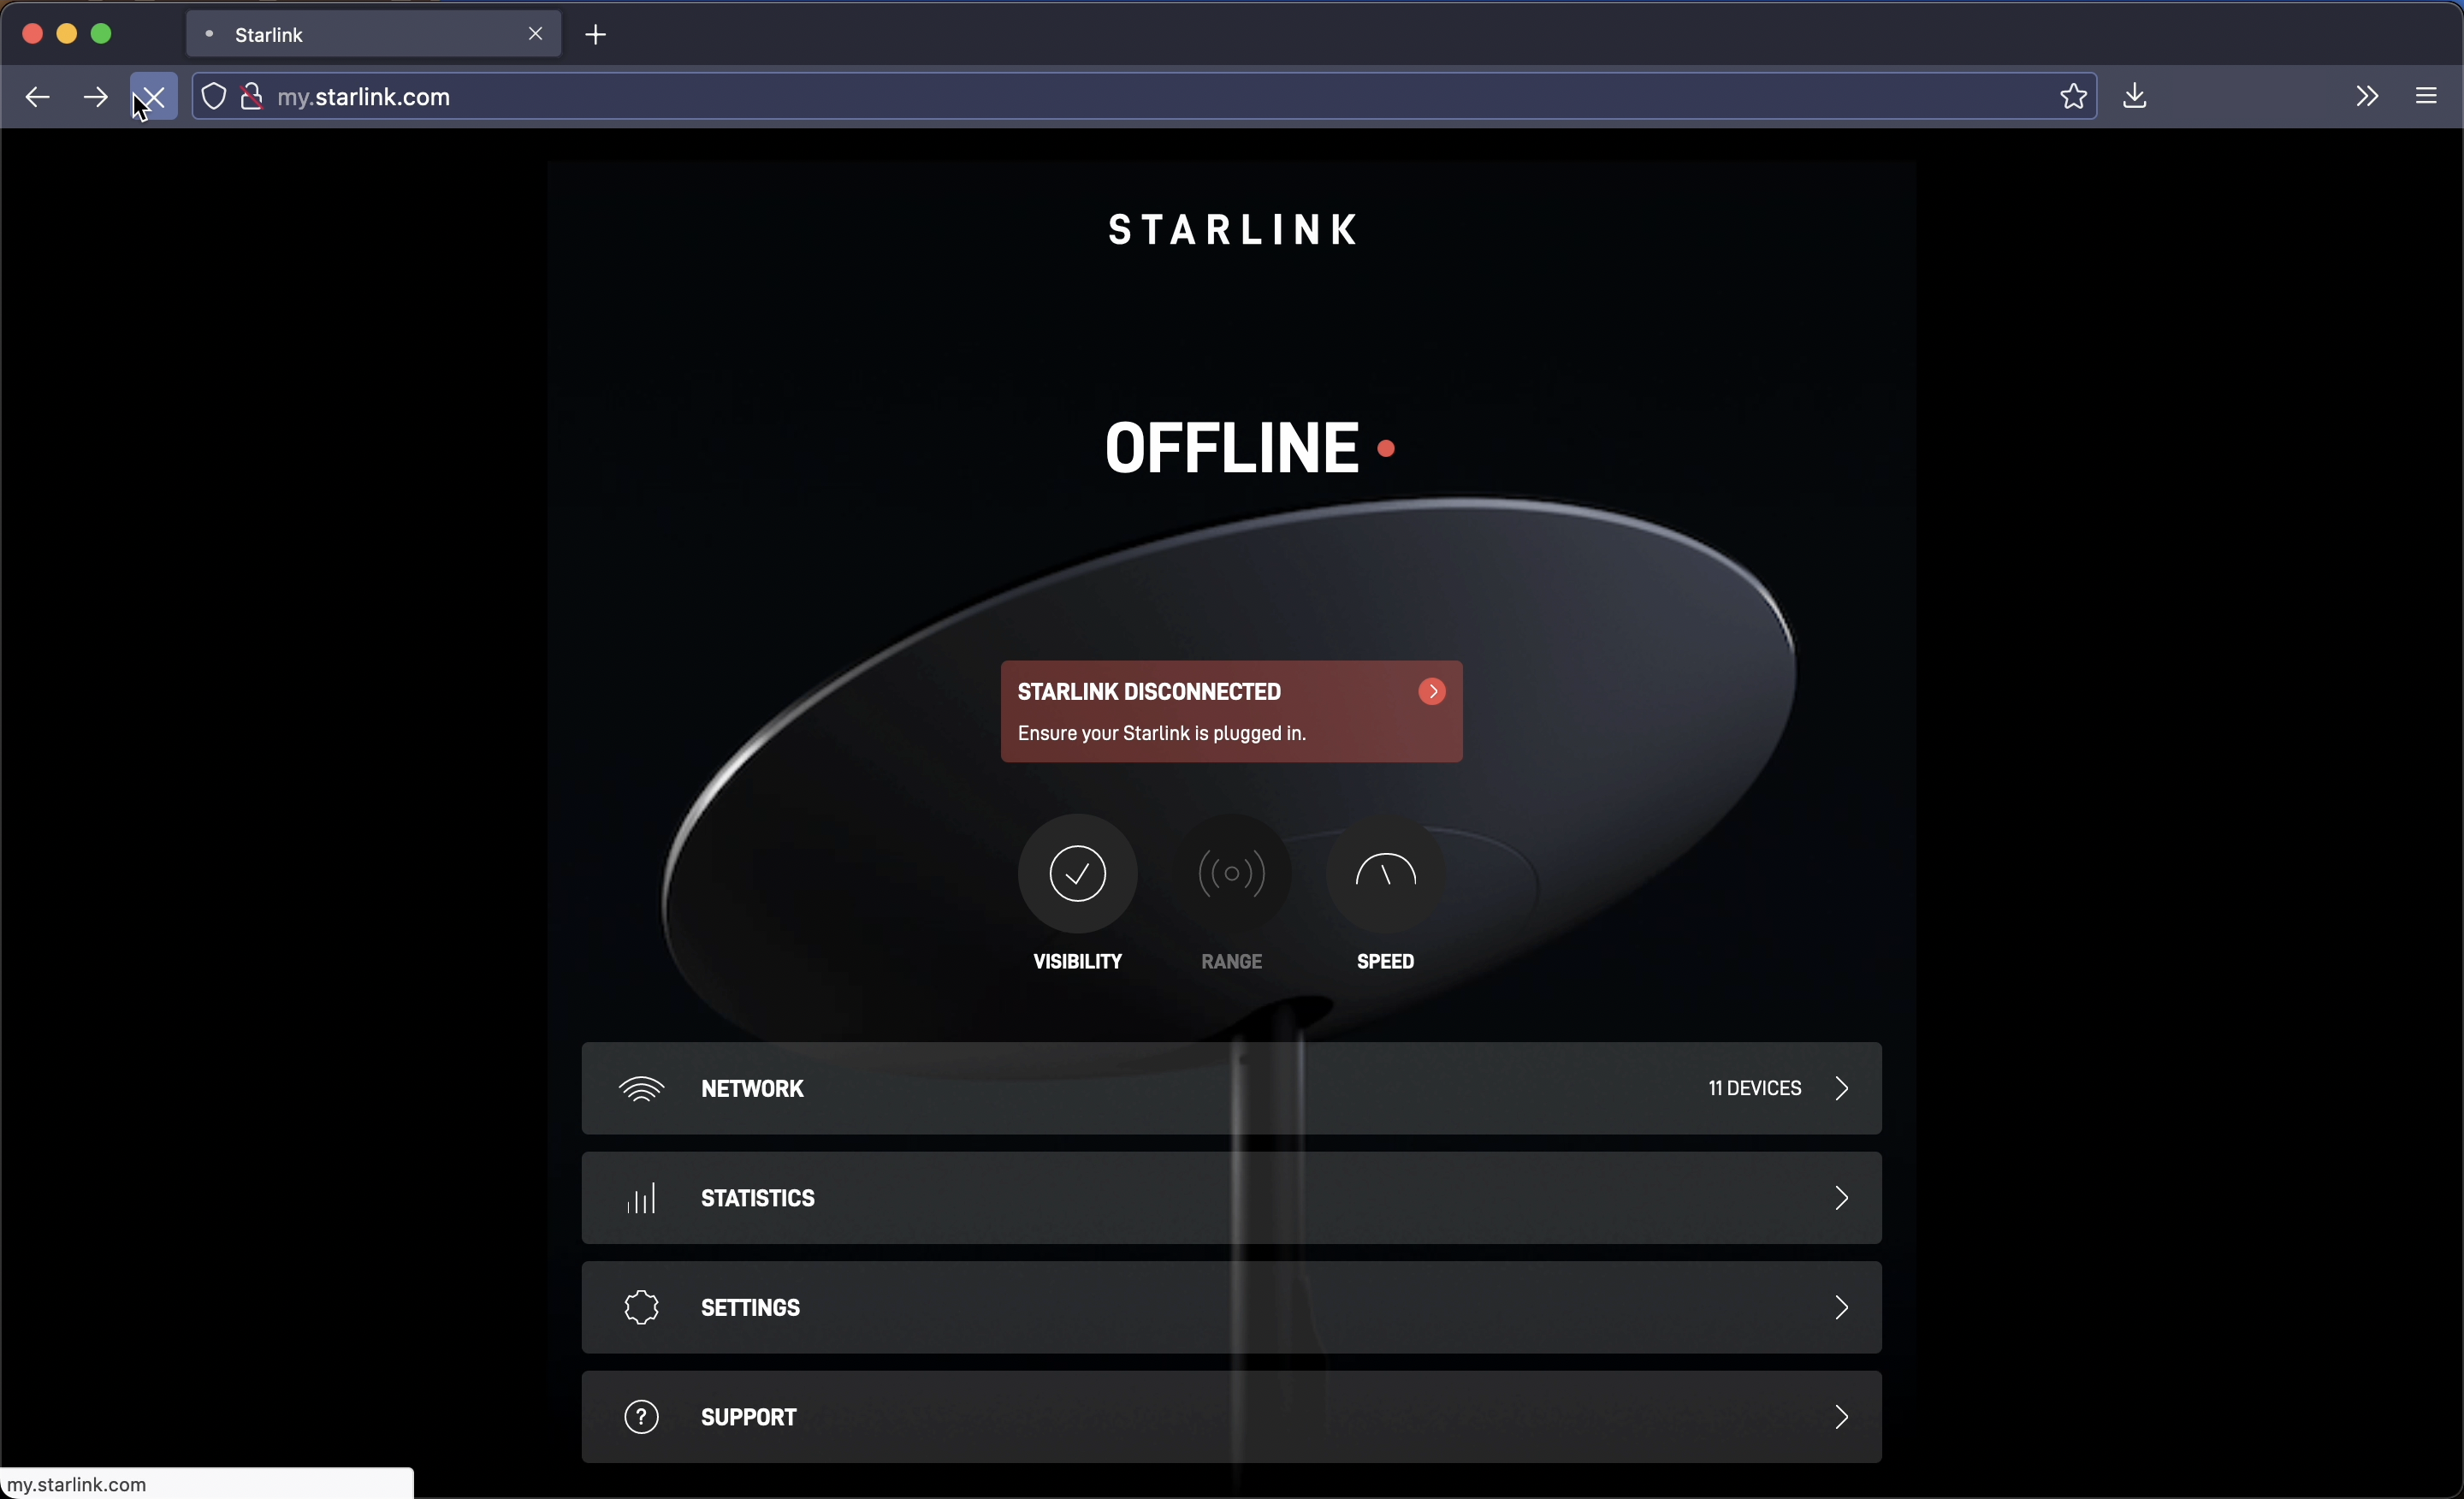
\includegraphics[width=\textwidth]{img/offline.png}\\\vspace{.35em}
        \centering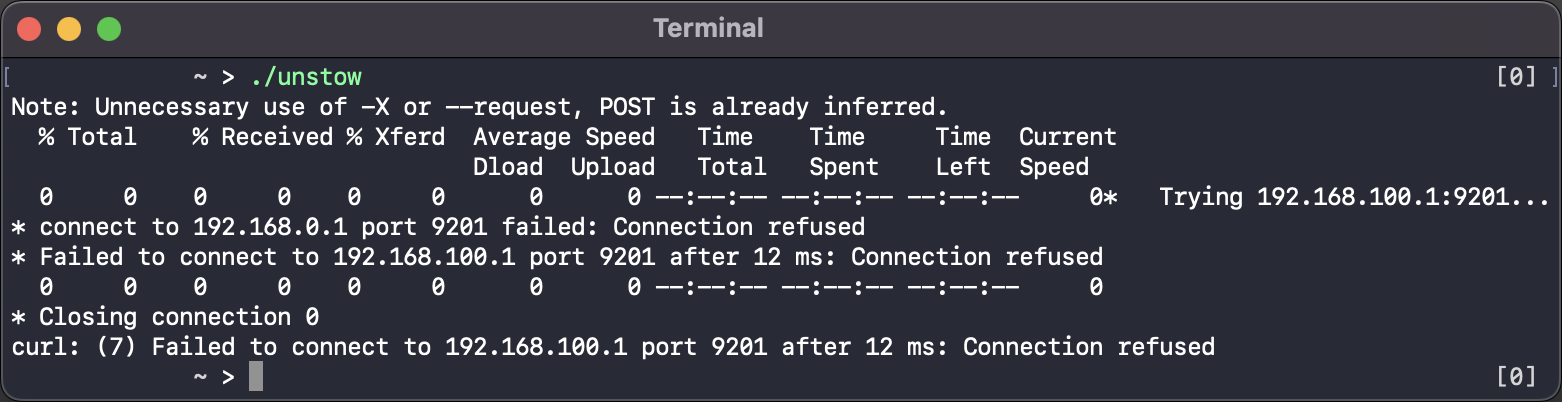
\includegraphics[width=\textwidth]{img/unstow.png}
        \caption{A screenshot of the web control panel error screen following the attack, and the result of sending commands to an inoperative dish.}
    \end{subfigure}
\caption{The outcome of a successful attack on the Starlink dish, and the resulting web control panel and response to commands.}
\label{fig:attack-outcome}
\vspace{-1.5em}
\end{figure*}

The Starlink user terminal is typically administered via the ``\url{http://my.starlink.com}'' web interface.
This sends commands to the modem over the local network, using gRPC (Google Remote Procedure Calls) encapsulated within HTTP ``POST'' requests.
As shown in Figure~\ref{fig:modem}, these requests are decoded by a gRPC web proxy, and forwarded to a command handler.

Although some gRPC commands require password authentication, the vast majority do not, including commands affecting the physical state of the dish.

Since the gRPC payload is usually between 2 and 5 bytes, the command space can be fuzzed with random contents to discover corner cases in the command handler which lead to unexpected behavior.
Through this we discovered the ``kill'' command \lstinline{00 00 00 00 03 EA 3E 00}, which causes the command handler of the user terminal to crash.

Since the modem will no longer respond to commands, the terminal is frozen in whatever state it was in before the kill command was sent.
An attacker can therefore lock the physical dish into a stowed state as seen in Figuree~\ref{fig:attack-outcome}, persistently denying service even after the attacker is no longer present on the network.
In this state, restoring internet access requires a physical power-cycle.
